\documentclass[nobib]{tufte-handout}

\usepackage{epigraph}
\usepackage{csquotes}
\usepackage{xcolor}
\usepackage{graphicx}
\usepackage{todonotes}
\makeatletter
\renewcommand{\subsubsection}{\ttl@straightclass{subsubsection}}
\makeatother
\titleformat{\subsubsection}[hang]
  {\selectfont\it}
  {\thesubsubsection}
  {1em}
  {}
  []
\newcommand{\placeholdertext}[1]{
	\noindent{\color{red}{#1}}
}

\newcommand{\CiteThis}{
({\color{red}{CITE THIS}})
}

\newcommand{\csharp}{c\#}

\title{Literature Review of Leading Research in Compiler Optimizations}
\author{Timothy Van Slyke}

\begin{document}
\maketitle
\section*{Abstract}
\todo{TODO: Many sections are currently just \textsf{lorem ipsum}'d and have yet to be written.  All other sections mainly consist of talking points.}
\begin{abstract}
\end{abstract}


%%% Introduction %%%
\section{Introduction}
\todo{TODO: Collapse some of the subsections directly into the introduction and just let the discussion flow on its own.}

\subsection{Rationale}
\begin{displayquote}
\textit{``Software is getting slower more rapidly than hardware becomes faster.''}
\newline\noindent\hfill{-- Niklaus Wirth} \\
\end{displayquote}
The modern software ecosystem is rich with a variety of platforms with distinct needs.  With the advent of mobile computing\footnote{Here we use the term ``mobile computing/platforms/devices'' to primarily refer to so-called ``smart devices'' such as smart phones and tablets.  While traditional mobile computing devices (i.e. laptops) face many of the same issues as smart devices, they share a fair number of similarities with desktop computers and may not appropriately be described by some of the generalizations discussed here.}, traditional software development practices have seen major disruptions over the past decade.  While the x86 architecture continues to dominate the desktop market, mobile platforms have largely adopted RISC\footnote{Reduced instruction set computer.} architectures; particularly, ARM-based CPUs.  Additionally, the widespread and international usage of social media platforms, web search engines, and other large-scale web services has necessitated an expanding usage of centralized data centers, or ``server farms''.  Both of these platforms, mobile devices and servers, despite having distinctly disparate use cases, make nearly identical demands from the software that they use.

\begin{itemize}
\item Both mobile devices and centralized data centers demand energy efficiency.
\end{itemize}
To quote Chandler Carruth, technical lead for Google's C++ and LLVM teams, ``The only thing [a data center does] is take electricity and turn it into heat.  That is its job.'' \CiteThis{}.  Maintenance of large-scale data centers present some of the largest expenses for firms such as Google, Amazon, Facebook, and other tech giants.  Improvements to the power usage of the software that runs on these servers present a major opportunity for engineers to reduce expenditures.  Similarly, mobile devices are constrained by the fact that they must employ a depletable power source.  Devices which are battery-operated also incentivize low power consumption, by necessity.

To date, the most effective strategy for reducing power consumption by computation has been to increase software speed \CiteThis{}.  CPUs have developed an impressive capacity for reducing energy usage via hibernation capabilities.  Modern advice in the software development community for increasing so called ``compute per Watt'' is to ``finish quickly so the device can go to sleep''.

Motivations for producing faster software are plentiful even when ignoring the energy consumption argument.  It would be hard to conceive of a scenario in which making a computer program slower is desired, and certainly such a task could not be difficult to achieve\footnote{It might be argued by some that the task of producing slower programs is a solved problem in modern software development.}.  In light of this universal need for faster software we seek to answer the following quesion:

\begin{displayquote}
What advancements in the state-of-the-art for compiler optimizations are being pursued in contemprory research?
\end{displayquote}




%% Background %%
\subsection{Background}
\placeholdertext{Discuss fact that CPUs are super complex and compilers know it.}
Modern optimizing compilers have matured for nearly half a century.  At a bare minimum, any serious optimizing compiler can be expected to be capable of some basic time.

What follows is a non-exhaustive list of what a can be expected from a modern compiler:
\begin{itemize}
\item Callsight-sensitive subroutine inlining.
\item Devirtualization. 
\item Copy elision.
\item Loop unrolling. 
\item Target-specific code generation.  
\item Common subexpression elimination.
\item Constant folding.
\item Primitive alias analysis. 
\item Dead code elimination.
\item Register allocation.
\end{itemize}

The above list could be expanded much further.  For example, the GNU Compiler Collection (GCC - originally the GNU C Compiler) is among the most well-known open-source compilers due to its long history of use in major projects like the Linux Kernel, and due to its portability.  Compilers like GCC have experienced decades of refinement and experimentation; such 

Recently the LLVM project has gained considerable traction as a general purpose compiler framework, and was the platform of choice for \placeholdertext{(list of sources that used LLVM to implement their experiments)}.  

More recent, compilers have begun supporting profile-guided optimization (PGO): a method which involves double compilation of a program.  The first compilation is used to produce an executable which is run through a profiling suite and collects profiling data.  This data is then fed back to the compiler during the second compilation which applises a series of more informed optimizations.  The success of PGO has proven that runtime information can have a major impact on program performance.

Much of modern research in the realm of optimizing compilation strategies revolves around the idea of leveraging information only known at runtime.  Many of the strategies explored in this review seek to leverage runtime information by applying aggressive code transformations that dynamically adapt according to the same kind of information found in the first compilation step of PGO.  The primary difference with that these methods is the elision of the need for recompilation.  

We explore the following trends in modern compiler optimization research:
\begin{itemize}
\item Non-trivial code generation aimed at adaptive runtime performance improvements.
\item State-of-the-art in ``traditional'' optimizations (local code improvements, instruction reordering, static analysis).
\item Automatic parallelization.
\end{itemize}

\placeholdertext{Desktop computing bottlenecked by memory latency} \newline
\begin{itemize}
\item There exist well-known cache-friendly access patterns but they don't always correspond with maintainable/readable code.
\end{itemize} 
\placeholdertext{Desktop computing bottlenecked by memory latency} \newline
\placeholdertext{Most if not all desktop-related rationale applies to servers.} \newline
\placeholdertext{Additionally, server farms face power consumption problems similar to those that faced by mobile platforms (but for different reasons).}
\placeholdertext{C programmers' expectations about code generation} \ldots

\placeholdertext{JIT compilation} \ldots
Just-in-time (JIT) compilation has become a major focus of many compiler projects due to the rise of managed languages like Java and \csharp in the past few decades.  JIT compilation complements a managed environment well 


Such platforms typically have reference semantics.  This hinders a compiler's ability to perform static (compile-time) alias analysis and implicitly hurts cache efficiency.  Reference semantics dictate that data is stored sparsely and accessing any data requires at least one indirection through a pointer.  JIT compilers have become a major player in this space because their ability to apply transformations at run time \placeholdertext{...}.

% Java Object Model
\begin{figure} 
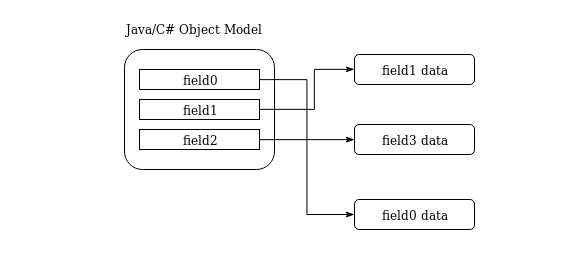
\includegraphics[width=\linewidth]{images/JavaObjectModel.png}
\caption{Visualization of the object model for languages with reference semantics.  Object fields are stored sparsely and object references are aliased liberally.  This leads to cache-unfriendly memory access patterns and poor conditions for alias analysis.}
\label{fig:JavaObjectModel}
\end{figure}




\begin{itemize}
\item Popular for VM runtimes.
\item Difficult for native code.
\end{itemize}


\placeholdertext{Cache latency is one of the largest factors in program speed} \ldots



%% Methods %%
\subsection{Methods}
We've analyze publications from \placeholdertext{LIST OF CONFERENCES} \ldots


%%% Modern Compiler Optimizations %%%
\section{Modern Compiler Optimizations}
Many of the optimizations made by modern comilers for static languages like C, C++, and Java are speculative and rely on making conservative and provable deductions.  


\subsection{Dynamic Runtime Solutions}
A common roadblock to many compiler optimizations is a lack of information at compile-time.  Certain information can only be known at runtime, for example: 
\begin{itemize}
\item The likelihood that a given conditional branch path will be taken.\footnote{Likely branches are typically called ``hot pathes''.}
\item Type information contained in dynamic libraries.
\item Buffer and dynamic array sizes.
\end{itemize}

This lack of information prevents compilers from making informed decisions about how local optimizations should be structured.  Managed languages like Java and \csharp have a built-in opportunity to leverage this information in the form of state-of-the-art JIT compiler techniques.  Languages which require a virtual machine bytecode interpreter typically provide JITs to improve performance by providing facilities to transform VM bytecode to machine code.  Compilers for specific VM runtime environments can implement efficient runtime facilities for dynamic code transformations since they ``own'' both the compiler and the VM.  This enables a larger class of optimizations for compilers because they can operate under the assumption that the unknown information can be collected at runtime.

Languages which are typically compiled directly to machine code (prominent examples being C, C++, and Rust) cannot make the same assumptions as managed languages.  Implementing such facilities would require inserting code for data collection and the correpsonding conditional code transformations without support from the runtime environment.  Additionally, and perhaps more importantly, such aggressive transformations are atypical and violate programmers' expectations about code generation.  

Nonetheless, research is being done in this area for both managed and unmanaged programming languages.  This research can largely be categorized into one of the following two categories:
\begin{itemize}
\item Significant code generation to collect and utilize drastically transform the behavior of the input source code (\placeholdertext{WHOMST?}).
\item Extending existing run-time JIT compilation techniques with new methods. (\placeholdertext{WHOMST'D?}).
\end{itemize}

Dissenga et al propose a framework for abstract interpretation 

\placeholdertext{Programmer-visible vs Programmer-invisible optimizations} \ldots \newline
\placeholdertext{Abstract Interpretation} \ldots \newline
\placeholdertext{Tracing JIT Compilation (recently combined with Abstract Interpretation Micro\$oft)} \ldots \newline




\subsubsection{Aggressive Code Generation in Unmanaged Languages}
While aggressive runtime solutions to compile-time problems have typcally revolved around JIT compilation in managed runtime environments, some authors have proposed dynamic methods in unmanaged languages such as C and C++.  

Lifflander and Krishnamoorthy show promising results when applying aggressive transformations to recursive programs in a fairly nonstandard fashion.  Proposed is a method for reorgranizing recursive\footnote{This method allows for indirect recursion of non-trivial depth.} subroutine calls into context switches between a series of lightweight user-level threads; showing comparable speeds with the PLuTo and Pochoir parallelizing compilers.  \placeholdertext{Doesn't scale too well though...}

%% Cache-Oriented Optimizations and Memory-Bound Code %%
\subsection{Cache-Oriented Optimizations and Memory-Bound Code}


Often the most important factor that determines the speed of software on modern computer systems is the extent to which the software is able to exploit the benefits CPU cache.\footnote{This factor is relevant on both desktop and mobile platforms.  Exceptions to this rule are microcontrollers and other very small systems.}  Much work is being done to speculatively optimize code for optimal memory access patterns and to reduce CPU stall time by rerdering and eliminating memory-bound operations.  Software prefetching, explicit instructions to hoist 

Software prefetching has shown promising results in benchmarks of otherwise cache-unfriendly code.  Experiments have shown anywhere from 2.1x to 2.7x performance improvements from compiler-generated prefetch instructions; competing well with "hand rolled" prefetch placement (Ainsworth et al) \CiteThis{}.  These promising results complement similar findings by Tran et al. who propose similar generative and transformative methods of cache locality improvements.  Tran et al. offer an instruction reordering framework which aims to improve access patterns with somewhat more conservative generation of software prefetch instructions \CiteThis{}.  Their methods more heavily rely upon dependency analysis to ensure correctness, but offer opportunities aggressive code transformations.  

Additional contributions aimed at improving cache performance come from the previously mentioned work by Lifflander and Krishnamoorthy \CiteThis{}.  Their dynamic splicing approach revolves around the assumption that lightweight thread context switches can offer better I-cache\footnote{Modern CPU caches typically segregate data and instructions in separate dedicated caches, respectively called the D-cache and I-cache.  Without qualification, the unqualified term ``cache'' typically refers to just the D-cache.} retention than traditional function calls.  There method reduces call stack usage and redundant function parameter copying by transforming recursive function calls into a coroutine-like usage pattern.  For each recursive call site, a user-level thread is spawned in place of pushing a new stack frame.  Subsequent invocations at that call site are then implemented as context switches to the already-existing thread.  Their method is limited in applicability by potentially intractable read-write patterns to shared data across spawned threads and introduces some overhead in the form of runtime \emph{effect annotations} and context switches. 

This method proposed by Lifflander and Krishnamoorthy takes an evidently different approach to those of Tran et al. and Ainsworth et al., most notably in the fact that the former result in significant runtime analysis and code generation while the latter are purely compile-time constructs.  Such research into dynamic methods have become more common in recent years and will likely continue to see more attention as memory latency effects continue to hinder software speed.  

\placeholdertext{Languages with reference semantics (Java, C\#, Python) suffer poor cache performance because of their implicit object model.} \ldots \newline
\begin{itemize}
	\item Every object is dynamically allocated. 
	\item Scattered data -- no control over allocation patterns or memory layout.
\end{itemize}

\todo{TODO: Move this discussion and associated visuals to introduction/background?} Optimizing comilers for these languages suffer from few opportunities for alias analysis and must fight an uphill battle when it comes to optimizing for cache-friendly access pattens.


% C++ Object Model
\begin{figure}
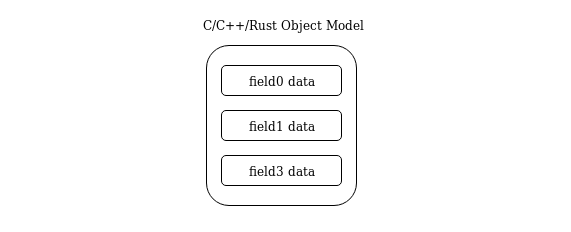
\includegraphics[width=\linewidth]{images/CppObjectModel.png}
\caption{Visualization of the object model for languages with value semantics.  Object fields are stored in a dense fashion and can only be aliased with explicit action in the code.  This leads to more cache-friendly memory access patterns and allows for reasonable alias analysis.}
\label{fig:CppObjectModel}
\end{figure}

% Python Object Model
\begin{figure}
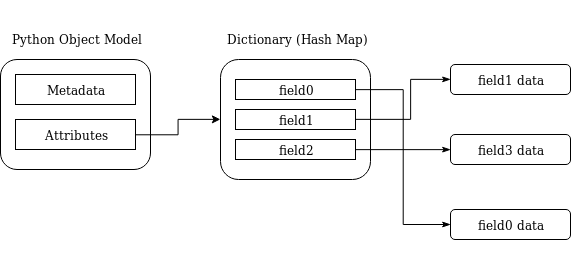
\includegraphics[width=\linewidth]{images/PythonObjectModel.png}
\caption{As a special case, the Python object model is, with only a few exceptions, implemented with a hash map; accessing object fields implies at least two layers of indirection.  This allows for highly dynamic code, but leads to extremely poor memory access patterns and makes compile-time alias analysis infeasable.} 
\label{fig:PythonObjectModel}
\end{figure}



\subsection{Model Improvements}
Some work has striven to improve compiler performance by considering novel internal representations of programs.  Mehta and Yew propose an polyhedral\footnote{Polyhedral (or polytope) compilation is a name given to a method of modeling nested loops to produce more optimization opportunities than traditional loop optimization techniques offer.} control-flow dependency model and present promising benchmark results in their experimentation.  Their contribution can be expressed as modelling data dependencies at block-level, rather than at the granularity of single statements.  This results in a model that produces a smaller dependency graph for larger-scale programs without sacrificing optimization oportunities.  They implement their model as an extension to the existing PLuTo polyhedral compiler and provide benchmarks which demonstrate a 1.92$\times$ performance gain over the best-performing, non-polyhedral compiler (Intel's ICC).  Additionally, their block-level dependency model implementation results in an astonishing 20-168$\times$ speedup over the vanilla PLuTo compilation procedure \CiteThis{}.

Additional model improvements are proposed by Ko et al. with a specialized IR\footnote{Intermediate representation; a language-agnostic representation of source code that optimizers apply transformations to.  IRs are converted to machine code in the final stages of compilation.} for FIFO\footnote{First in, first out.} streams.  More precisely, the proposed IR is shown to improve performance over FIFO compile-time stream models with an implementation using the LLVM compiler framework.  Their benchmarks with LaminarIR demonstrate an average speedup of 1.56$\times$ over the traditional FIFO model, and a 1.34$\times$ speedup over the StreamIt compilation framework \CiteThis{}.

The drastic gains demonstrated by ongoing research in internal compiler models show promise for specialized compilation techniques.



\subsection{Optimizing Parallel Code}
\placeholdertext{Automatic parallelization of code} \ldots \newline
\placeholdertext{Optimization of synchronization schemes} \ldots \newline

\subsection{Misc. or Yet-To-Be-Named Section}
\placeholdertext{Alias analysis} \ldots \newline
\placeholdertext{} \ldots \newline

\section{Results}

\section{Conclusions}



\newpage
\nocite{*}
\bibliographystyle{IEEEannot}
\bibliography{annot}




\end{document}

